% !TeX root=../main.tex

\ifdefined\DEBUG
\newcommand{\unravelled}{unravelled}
\newcommand{\unravelling}{unravelling}
\newcommand{\unravel}{unravel}
\else
\newcommand{\unravelled}{unfolded}
\newcommand{\unravelling}{unfolding}
\newcommand{\unravel}{unfold}
\fi

%\def\WWITHN{def}
\ifdefined\WWITHN
\newcommand{\WCal}[2]{{\mathcal{W}_{#1}^{#2}}}
\newcommand{\TBf}[2]{{\mathbf{T}_{#1}^{#2}}}
\else
\newcommand{\WCal}[2]{{\mathcal{W}_{#1}}}
\newcommand{\TBf}[2]{{\mathbf{W}_{#1}}}
\fi


\subsection{Alignment Strategy}
\texttt{\color{red}[MEMO: ``unfolded trace'' can be omitted, as trace should already\\ refer to unfolded traces]}.
Trace alignment algorithms usually provide as output a single alignment for a single model trace. However, in practice, approaches generating different alignment possibilities would provide the user with a richer feedback. This is even more important for approaches based o stochastic nets, like USWNs, since, in this case, distinct model traces have different probabilities and the retrieval of the best model trace maximizing the combined provision of minimum trace alignment cost and maximum model trace probability might not suffice. Therefore, we would
like to return the best $k$ alignments among all the distinct \unravelled\ model traces in $\WCal{p_\theta}{n}(P)$. In the database community, this problem is usually tackled via $k$-Nearest Neighbors.

The well-known $k$-nearest neighbors ($k$NN) problem \cite{Altman} refers to finding the $k$ nearest data points to a \textit{query} $x$ from a set $\mathcal{X}$ of \textit{data points} via a distance function $d_k$ defined over $\mathcal{X}\cup\{x\}$. Usually, $x$ and $\mathcal{X}$ are represented as numerical vectors via an embedding $\phi$. {By exploiting ad-hoc data structures such as Vp-Trees \cite{Fu2000}, Kd-Trees \cite{Maneewongvatana99}, and M-Trees \cite{Ciaccia}, we can retrieve the neighborhood of $x$ in $\mathcal{X}$ of size $k$  by pre-ordering (\textit{indexing}) $\mathcal{X}$  via $d_k$. Thus, we do not need to analyze the entire space, but just start the search from the top-$1$ alignment. We prefer embeddings $\phi$ for $\mathcal{X}$ that are independent from the query of choice $x$, as it would not require to constantly change the numeric vector representation for $\mathcal{X}$.
%	
If we want to align the trace $\sigma^*$ over the \unravelled\ traces $\mathcal{X}=\WCal{p_\theta}{n}(P)$ and $d$ is a distance, the $k$-nearest neighbors describe the best $k$ alignments for $\sigma^*$.} We now discuss two different possible strategies for obtaining the top-$k$ model trace alignments.

\subsubsection{Optimal-Ranking Trace Aligner}\label{subsec:eta}
{A possible way to carry out probabilistic trace alignment is to reuse existing trace aligners such as \cite{LeoniM17}, where the notion of distance $d(\sigma,\sigma^*)$ between two traces $\sigma$ and $\sigma^*$ (introduced in \S\ref{subsec:katk}) is the Levenshtein distance, i.e., the \ADD{minimum} cost for aligning one of the two traces with respect to the other when all the possible moves have cost equal to 1.\footnote{This distance is slightly different from the Levenshtein distance known in the literature since here the replacement is obtained as a concatenation of a deletion and an addition.} We can then exploit decision theory \cite{dectheor} and express the statistical decision of aligning a weighted trace $\braket{\sigma,w_\sigma}\in\WCal{p_\theta}{n}(P)$ with $\sigma^*$ as the $w_\sigma$-weighted distance between the two traces, i.e., as $w_\sigma d(\sigma,\sigma^*)$, and rank the alignments based on this metric (this produces what we call an \emph{optimal ranking}).

If we want to represent the same intuition of such a weighted distance as a kernel function (\S\ref{subsec:katk}) so to compare the optimal-ranking strategy to our proposed approximate-ranking trace embedder, we need to transform it as a similarity function returning $1$ when $\sigma=\sigma^*$ and has probability $w_\sigma=1$. We then express $d$ as}
%\xout{We can express our probabilistic trace alignment as finding the trace that maximizes both the trace's probability and its similarity with the query trace $\sigma^*$. Still, the trace alignments problems are usually expressed via trace alignments cost functions, and not via trace similarities \cite{LeoniM17}. Given a generic trace cost function $d(\sigma,\sigma')$, it is always possible to convert it into}
a normalized similarity score $s_d(\sigma,\sigma'):=1/(d(\sigma,\sigma')/c+1)$ where $c\in\mathbb{N}_{\neq 0}$ is a constant, so that the maximum similarity of $1$ is reached when the distance is $0$ and the similarity decreases while the distance increases \cite{BergamiBM20}. %\xout{As a consequence, the exact trace aligner will find the weighted trace $\braket{\sigma,\mathbb{P}(\sigma)}$ in $\mathcal{W}_{p_\theta}(P)$ maximising $s_d(\sigma,\sigma^*)$, and use $s_d$ as a ranking function.} \ADD
{Considering that if we interpret the trace to be aligned $\sigma^*$ as a TG, it is reasonable to assume that $w_{\sigma^*}=1$, we can express the golden kernel function (i.e., the one producing the optimal ranking) as $k_\star(\sigma,\sigma^*)=w_\sigma w_{\sigma^*} s_d(\sigma,\sigma^*)$. At this stage, the computation of $\underset{\braket{\sigma,w_\sigma}\in \WCal{p_\theta}{n}(P)}{\max\arg} k_\star(\sigma, {\sigma^*})$ returns the best optimal-ranking trace alignment $\sigma$ for a query trace $\sigma^*$, where $k_\ast$ must be computed a-new for all the possible $\sigma^*$ to be aligned.
	
	
	

\subsubsection{Approximate-Ranking Trace Embedder}\label{subsec:ate}
As previously observed, ranking optimality comes at the cost of a brute-force recomputation of all the embeddings $\phi$ for each novel trace $\sigma^*$ to align\footnote{By embedding  all the \unravelled\ model traces via $\phi_{\sigma^*}(\braket{\sigma,w_\sigma})=\Big(\frac{1}{w_\sigma\sqrt{w_\sigma^2+s_d^2(\sigma,\sigma^*)}},\frac{1}{s_d(\sigma,\sigma^*)\sqrt{w_\sigma^2+s_d^2(\sigma,\sigma^*)}}\Big)$ over a specific $\sigma^*$, by representing all the $\sigma^*$ as $(0,0)$, and by using the Euclidean Distance as a distance, we ensure that all the neighbors of $(0,0)$ will represent the top-$k$ best alignments for $\sigma^*$.}. This is not optimal for $k$NN-based techniques, as this entails the  redefinition of the multidimensional search space $\mathcal{X}$ for each new alignment $\sigma^*$. The ``recomputation cost'' could be completely avoided by providing an embedding strategy $\phi_{\mathcal{P}}$ that is independent from the to-be-aligned trace $\sigma^*$. Given that each embedding $\phi$ entails an associated similarity metric $k_\phi$ (\S\ref{subsec:katk}) and therefore an associated distance $d_{k_\phi}$ (Equation \ref{eq:dofk}), we can compute all the embeddings $\phi_{\mathcal{P}}$ for all the \unravelled\ traces before performing the top-$k$ search, thus avoiding the brute-force cost. This computational gain comes with a loss in precision, as the generation of precise embeddings for graph data with loops is an NP-Complete (thus intractable) problem \cite{GartnerFW03} and, in its approximated version, is not able to accurately represent the data using low-dimensional vectors \cite{Seshadhri5631}. So, our proposed definition of $\phi_{\mathcal{P}}$ performs  weakly-ideally (\S\ref{subsec:katk} and \cite{Gartner03}).

\ADD{The embedding strategy} $\phi_{\mathcal{T}}$ (\S\ref{subsec:katk} and \cite{LodhiSSCW02,Raedt}9 \ADD{from current literature has several short\-comings: firstly,} \begin{alphalist} \item it does not perform weakly-ideally, so we cannot numerically assess when two embedding represent equivalent traces (Example \ref{ex:wheredotiszero}). Secondly, \item it does not characterize $\tau$-moves, so initial $\tau$-moves' probabilities are not preserved (Example \ref{ex:neue}). Thirdly, \item it is affected by numerical errors from finite arithmetics (e.g., double, float): longer traces $\sigma$ generated from skewed probability distributions $\Lambda^i$ will suffer from greater truncation errors, as smaller $\lambda^i$ components for bigger $i<|\sigma|$ will be ignored, thus preventing a complete numerical vector characterization of  $\sigma$ in practice.
\end{alphalist}

\ADD{We overcome these shortcomings by} \begin{alphalist} \item proposing a weakly-ideal embedding (p. \pageref{subsub:prop}), which also \item exploits an $\omega$ factor for preserving probabilities from and to $\tau$ transitions (Example \ref{ex:neue}). Furthermore, \item we mitigate the numerical truncation errors induced by trace length and probability distribution's skewness by introducing two sub-embedding strategies, $\epsilon^x$ and $\nu^x$, where the former descends from $\phi_{\mathcal{T}}$ and the latter approximates the trace similarity via label frequencies' similarity.
\end{alphalist}

Given that the embedding of a (weighted) trace $\braket{\sigma,w_\sigma}\in\WCal{p_\theta}{n}(P)$ requires an intermediate $TG$ representation, we can map each of these traces to the subgraph of $P$ generating $\braket{\sigma,w_\sigma}$ with at most $|\sigma|$ steps:}
	\begin{definition}[TG projection over traces]
		Given a minimum probability threshold $p_\theta$, a maximum path length $n$, and a TG $P=(s,t,L,R,\omega)$, we generate a set $\TBf{p_\theta}{n}(P)$ of projected TGs $P$ for each trace in $\WCal{p_\theta}{n}(P)$ as follows: for each weighted trace $\braket{\sigma,w_\sigma}\in\WCal{p_\theta}{n}(P)$ generated from a path $\pi_\sigma=s\to n_2\rightsquigarrow n_m\to t$ over $R$, we generate a TG $P_\sigma=(s',t',L_\sigma,R_\sigma,\omega')$, where \begin{alphalist}
			\item $s'=s$ if $\textit{label}(s)\neq \tau$ and $t'=n_2$ otherwise,
			\item $t'=t$ if $\textit{label}(t)\neq \tau$ and $t'=n_m$ otherwise,
			\item $L_\sigma$ (and $R_\sigma$) is the submatrix of $L$ (and $R$) over the non-$\tau$ labeled notes in $\pi_\sigma$ and the labels from $\sigma$,
			\item $\omega'$ is initialized by $\omega$ and then multiplied by $[R]_{s,n_2}$ (and also $[R]_{n_m,t}$) if $\textit{label}(s)=\tau$ (and  $\textit{label}(t)=\tau$).
		\end{alphalist}
	\end{definition}

\begin{table}[!t]
	\caption{Generating the sub-TGs $P_\sigma\in \TBf{\varepsilon}{4}(P)$ from the TG $P$ via the set of weighted traces $\WCal{\varepsilon}{4}(P)$, where $\varepsilon$ is the machine epsilon. $l$ and $w$ respectively represent the desired parameter for $\phi_{\mathcal{P}}(P_\sigma)$ and the weight associated to $P_\sigma$.}\label{tab:proj}
	\centering
	\resizebox{.45\textwidth}{!}{\begin{tabular}{>{\centering\arraybackslash} m{1cm}| >{\centering\arraybackslash} m{4cm} >{\centering\arraybackslash} m{1cm} >{\centering\arraybackslash} m{1cm} }
			\toprule
			$\sigma$&$P_\sigma$&$l$&$\omega$\\
			\midrule
			a & 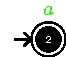
\includegraphics{images/trace_a} & $1$ & $\color{violet}\pa\pf$\\
			cb & 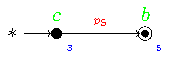
\includegraphics{images/trace_cb} & $2$ & $\color{violet}\pb$\\
			aaa & 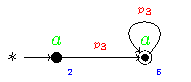
\includegraphics{images/trace_a_loop} & $3$ & $\color{violet}\pa\pf$\\
			caa & 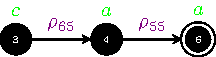
\includegraphics{images/trace_caa} & $3$ & $\color{violet}\pb\pf$\\
			\bottomrule
	\end{tabular}}\quad 	\resizebox{.45\textwidth}{!}{\begin{tabular}{>{\centering\arraybackslash} m{1cm}| >{\centering\arraybackslash} m{4cm} >{\centering\arraybackslash} m{1cm} >{\centering\arraybackslash} m{1cm} }
	\toprule
	$\sigma$&$P_\sigma$&$l$&$\omega$\\
	\midrule
	aa & 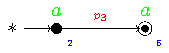
\includegraphics{images/trace_aa} & $2$ & $\color{violet}\pa\pf$\\
	ca & 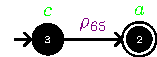
\includegraphics{images/trace_ca} & $2$ & $\color{violet}\pb\pf$\\
	\begin{tabular}{l}aaaa\end{tabular} & 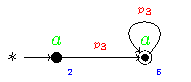
\includegraphics{images/trace_a_loop} & $4$ & $\color{violet}\pa\pf$\\
	caaa & 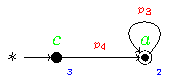
\includegraphics{images/trace_ca_loop} & $4$ & $\color{violet}\pb\pf$\\
	\bottomrule
\end{tabular}}
\end{table}
\begin{example}\label{ex:neue}
Given the TG $P$ in Figure \ref{fig:closed}, we assign the following probability values to the edges: $\pa=0.8$, $\pb=0.2$, $\pc=\pf=0.5$, $\pd=0.7$, and $\pe=0.3$. If we limit our analysis to all the traces of maximum length $4$, we generate the following probabilistic traces set:
$$\begin{aligned}
\WCal{\varepsilon}{4}(P)=\{&\braket{a,0.4},\braket{aa,0.2},\braket{aaa,0.1},\braket{ca,0.07},\\
&\braket{cb,0.06},\braket{aaaa,0.05},\braket{caa,0.035},\braket{caaa,0.0175}\}\\
\end{aligned}$$
\medskip

Table \ref{tab:proj} represents the TGs $P_\sigma\in\TBf{\varepsilon}{4}(P)$ with weight $\omega$ generated for each weighted path $\braket{\sigma,w_\sigma}\in \WCal{\varepsilon}{4}(P)$ of length $l=|\sigma|$ from the TG $P$ in Figure \ref{fig:closed}. The associated weight $\omega$ derives from the source's outgoing edges (and target's ingoing edges) when such node is labeled as $\tau$: given that both \textbf{(i)} the embedding strategy from current literature (\S\ref{subsec:katk}) allows trace embedding just for visible (i.e., non-$\tau$) transitions, and that \textbf{(ii)} such trace extraction process discards the $\tau$ information but we want to preserve the transition probabilities from and to $\tau$ transitions, we exploit an additional parameter $\omega$ to preserve such information.
%\xout{selection of a trace $\sigma$ implies performing a set of specific probabilistic choices, we can remove all the edges starting (and arriving) at nodes that are $\tau$-labelled and move their score as the weight of the TG.}
\end{example}
	
{We can now focus on the embedding $\phi_{\mathcal{P}}$ for each TG associated to our selected weighted traces. The main goal is to use $k_{\phi_\mathcal{P}}$ for ranking all the traces generated by the \unravelling step. Walking on such footsteps, we  want to extend  previous work on embeddings (\S\ref{subsec:katk}) by both including the traces' associated probability and by making the ranking induced by $k_{\phi_\mathcal{P}}$ the inverse of the ranking induced by the sum of the following distances: the transitions correlations $\epsilon$ and the transitions label frequency $\nu$ ({Proof omitted due to lack of space}). }
%\xout{Given that we previously observed that a TGs $P$ can be fully characterised (read, similarity) by their associated set of traces $\mathcal{W}_p^n(P)$  and that the trace embedding can be described as an embedding over a TG, we can characterise a TG embedding as a transition matrix embedding. In addition to that, when two Workflow Nets share similar node labellings but no ${\color{green}\alpha}\rightsquigarrow{\color{green}\beta}$ paths for any ${\color{green}\alpha}$ and ${\color{green}\beta}$, we should combine the former embedding with an embedding characterising the frequency on how the nodes' labels appear in the generated traces.} \ADD
{We also require that the desired properties of $\phi_{\mathcal{P}}$ are independent from the characterization of $\epsilon$ and $\nu$, which  provide different embedding strategies. } The final embedding is defined as follows:


%\begin{table}[!t]
%	\centering
%	\caption{Embedding representation for the TG $P$ in Figure \ref{fig:closed} and the trace $\sigma^*=\textup{caba}$ after representing it as in Figure \ref{fig:sigmastar}. Please note that we restrict $\Sigma_\tau^2$ to the one from $P$.}\label{tab:emb1}
%		\begin{tabular}{l|l|l|l|l|l|l|}
%	\toprule
%	& a    & b                                                   & c    & aa   & ca   & cb   \\
%	\midrule
%	$\phi_{\mathcal{P}}(P)$ & $9.94\cdot10^{-25}$ & $1.18\cdot 10^{-26}$ & $1.04\cdot10^{-25}$ & $4.45\cdot 10^{-25}$ & $6.22\cdot10^{-25}$ & $8.29\cdot10^{-26}$\\
%	$\phi_{\mathcal{P}}(P_{\sigma^*})$ & $8.16\cdot10^{-17}$ & $4.08\cdot 10^{-17}$ & $4.08\cdot10^{-17}$ & $4.37\cdot 10^{-17}$ & $1.03\cdot10^{-16}$ & $4.37\cdot10^{-17}$\\
%	\bottomrule
%\end{tabular}
%\end{table}
\begin{definition}[TG Embedding]\label{def:ppne}
Given a finite set of non-empty labels $\Sigma_\tau =\Sigma\backslash\{\tau\}$, $\Sigma_\tau^2$ denotes all the possible pair of labels associated to paths ${\color{green}\alpha}\rightsquigarrow{\color{green}\beta}$ and $\Sigma_\tau$ denotes the set of all the possible non-$\tau$ node labels. Therefore, it is always possible to enumerate $\Sigma_\tau^2\cup\Sigma_\tau$ via an enumeration by a bijection $\iota\colon \Sigma_\tau^2\cup\Sigma_\tau\to  N$, where $N\subset \mathbb{N}_{\neq 0}$ and $\max N=|N|$.
	
Given a TG $P=(s,t,L,R,w)$ resulting from a $\tau$-closure and a tuning parameter $t_f\in[0,1]\subseteq\mathbb{R}$, the associated embedding is defined as follows:
$$\phi_{\mathcal{P}}(P)_i=\begin{cases}
	\frac{\epsilon(P)_{\color{green}\alpha\beta}}{\|\epsilon\|_2}\omega t_f^{|R>0|} & i={\color{green}\alpha\beta}\\
	\frac{\nu(P)_{\color{green}\alpha}}{\|\nu\|_2}t_f^{|R>0|} & i={\color{green}\alpha}\\
\end{cases}$$
where $\epsilon$ and $\nu$ respectively represent the non-negatively defined embedding associated to the TG's transition matrix and nodes.
\end{definition}

At this stage, the computation of $\underset{\braket{\sigma,w_\sigma}\in \WCal{p}{n}(P), P_\sigma\in\TBf{p}{n}(P)}{\max\arg} k_{\phi_\mathcal{P}}(P_\sigma, P_{\sigma^*})$ returns the best approximated trace alignment $\sigma$ for a query trace represented as $P_{\sigma^*}$. %\xout{Similarly, we can provide the TG $P\in\mathbf{P}$ providing the best approximated alignment for $P_{\sigma^*}$ as $\underset{P}{\max\arg}\underset{ P_\sigma\in\mathbf{P}_p^n(P)}{\max} k_{\phi_\mathcal{P}}(P_\sigma, P_{\sigma^*})$.}¯

\begin{table}[!t]
	\caption{Different sub-embedding definitions ($\epsilon^1$, $\epsilon^2$, $\nu^1$, and $\nu^2$) for $\phi_{\mathcal{P}}$.}\label{tab:embedstrat}
	\centering
	\begin{tabular}{c|c|c}
		\toprule
		& $x=1$ & $x=2$ \\
		\midrule
		$\epsilon^x(P)_{\color{green}\alpha\beta}:=$ & $\label{eq:epsilon}
		\sum_{i=1}^l{\lambda^i}\frac{[LR^iL^t]_{\color{green}\alpha\beta}}{\sum_{\color{green}\alpha'\beta'}R^i_{\color{green}\alpha'\beta'}}$ & $
		\sum_{i=1}^l\lambda^i[\Lambda^i]_{\color{green}\alpha\beta}$\\
		$\nu^x(P)_{\color{green}\alpha}:=$ & $\frac{1}{N}\sum_{\braket{\sigma,w}\in\WCal{p}{l}(P)}\frac{|\Set{\sigma_i\in\sigma|\sigma_i\neq\tau\wedge \sigma_i={\color{green}\alpha}}|}{|\sigma|}$ & $0$ \\
		\bottomrule
	\end{tabular}
\end{table}
Albeit we might pick different characterizations for $\epsilon$ and $\nu$, {in our experiment section} we choose two possible interchangeable definitions ($x=1$ and $x=2$) for both sub-embeddings (Table \ref{tab:embedstrat}): $l$ is the path length indicated in Table \ref{tab:proj}, and $N$ for $\nu^1$ is a normalization factor such that $\sum_{{\color{green}\alpha}\in\Sigma_\tau}\nu^1(P)_{\color{green}\alpha}=1$. \ADD{While $\nu^2$ implies to completely ignore the label's frequency contribution, $\epsilon^2$ is the direct implementation of $\phi_{\mathcal{T}}$ from \S\ref{subsec:katk}, and $\epsilon^1$ and $\epsilon^2$ only differ from the normalization perspective.} %In Example \ref{ex:cmpexample}, we will see that the given definition of $\epsilon^1$ provides a better approximation than the edge embedding $\epsilon^2$.


%When the transition matrix is ergodic \cite{StocasticCC},  the transition matrix embedding converges to $\epsilon(R)_{\color{green}\alpha\beta}=[(\mathbf{I}-\lambda\Lambda)^{-1}]_{\color{green}\alpha\beta}$ \cite{GartnerFW03} for $n\to+\infty$.

\begin{table}[!t]
	\centering
	\caption{Embedding for both the traces $\sigma$ of maximum length $4$ from $P$ and  $\sigma^*$.}\label{tab:emb2}\label{tab:embsitar}
	\begin{tabular}{l|l|l|l|l|l|l|}
		\toprule
		& a    & b                                                   & c    & aa   & ca   & cb   \\
		\midrule
		
		
		$\phi_{\mathcal{P}}(P_\textup{aaaa})$ & $1.00\cdot 10^{-24}$ & $0.00\cdot 10^{0}$ & $0.00\cdot 10^{0}$& $6.44\cdot 10^{-26}$& $0.00\cdot 10^{0}$& $0.00\cdot 10^{0}$\\
		$\phi_{\mathcal{P}}(P_\textup{aaa})$ & $1.00\cdot 10^{-24}$ & $0.00\cdot 10^{0}$ & $0.00\cdot 10^{0}$& $1.29\cdot 10^{-25}$& $0.00\cdot 10^{0}$& $0.00\cdot 10^{0}$\\
		$\phi_{\mathcal{P}}(P_\textup{aa})$ & $1.00\cdot 10^{-24}$ & $0.00\cdot 10^{0}$ & $0.00\cdot 10^{0}$& $2.57\cdot 10^{-25}$& $0.00\cdot 10^{0}$& $0.00\cdot 10^{0}$\\
		$\phi_{\mathcal{P}}(P_\textup{a})$ & $1.00\cdot 10^{-4}$ & $0.00\cdot 10^{0}$ & $0.00\cdot 10^{0}$& $0.00\cdot 10^{0}$& $0.00\cdot 10^{0}$& $0.00\cdot 10^{0}$\\
		$\phi_{\mathcal{P}}(P_\textup{caa})$ & $7.07\cdot 10^{-25}$ & $0.00\cdot 10^{0}$ & $7.07\cdot 10^{-25}$& $1.46\cdot 10^{-25}$& $2.05\cdot 10^{-25}$& $0.00\cdot 10^{0}$\\
		$\phi_{\mathcal{P}}(P_\textup{ca})$ & $7.07\cdot 10^{-25}$ & $0.00\cdot 10^{0}$ & $7.07\cdot 10^{-25}$& $0.00\cdot 10^{0}$& $1.00\cdot 10^{-8}$& $0.00\cdot 10^{0}$\\
		$\phi_{\mathcal{P}}(P_\textup{cb})$ &  $0.00\cdot 10^{0}$ & $7.07\cdot 10^{-25}$ & $7.07\cdot 10^{-25}$& $0.00\cdot 10^{0}$&  $0.00\cdot 10^{0}$ & $4.29\cdot 10^{-9}$\\
		$\phi_{\mathcal{P}}(P_\textup{caaa})$  & $7.07\cdot 10^{-25}$ &  $0.00\cdot 10^{0}$ & $7.07\cdot 10^{-25}$& $1.03\cdot 10^{-25}$&  $7.20\cdot 10^{-26}$ & $0.00\cdot 10^{0}$\\
		\bottomrule
				$\phi_{\mathcal{P}}(P_{\sigma^*})$ & $8.16\cdot10^{-17}$ & $4.08\cdot 10^{-17}$ & $4.08\cdot10^{-17}$ & $4.37\cdot 10^{-17}$ & $1.03\cdot10^{-16}$ & $4.37\cdot10^{-17}$\\
		\bottomrule
	\end{tabular}
\end{table}
\begin{example}\label{ex:withpaths} After generating all the TGs for the \unravelled\ traces (Example \ref{ex:neue}), we further associate a sub-embedding $\epsilon$ using the $2$-grams included in the model traces.\footnoteref{fn:caveat}
Given $\Sigma_\tau=\Set{a,b,c}$, the embedding space is of size $6$: three features (computed using $\nu$) correspond to the labels of the non-$\tau$ vertices in $\Sigma_\tau$, i.e., $\{a,b,c\}$, and other three features (computed using $\epsilon$) correspond to the $2$-grams subsequences that are also traces in $W^4_0(P)$, i.e., $\{aa,ca,cb\}$. Therefore, $\{a,b,c,aa,ca,cb\}\subset \Sigma_\tau^2\cup\Sigma_\tau$ is the whole set of features describing both the label and the transition matrix, so $\phi_{\mathcal{P}}$ is a vector with 6 dimensions.
$t_f\in [0,1]\subset\mathbb{R}^+_{0}$ and $\lambda\in [0,1]\subset\mathbb{R}^+_{0}$ are tuning parameters that can be inferred from the available data \cite{DriessensRG06}. While the latter describes the previously mentioned decay factor, $t_f$ represents the relevance of our embedding representation when the number of the edges within TG increases. In both our experiments and examples, we chose $t_f=0.0001$ and $\lambda=0.07$.
%\xout{The embedding associated to $P$ is described in Table \ref{tab:emb1} as $\phi_{\mathcal{P}}(P)$: it shows that doing ${\color{green}a}\rightsquigarrow{\color{green}a}$ is more probable than doing  ${\color{green}c}\rightsquigarrow{\color{green}a}$. Also, given that both the probability of performing ${\color{green}c}\overset{1}{\rightsquigarrow}{\color{green}b}$ is relatively low and trace $\color{green}cb$ is relatively infrequent, ${\color{green}c}{\rightsquigarrow}{\color{green}b}$ is less probable than any other subtrace. If we now consider the single nodes, $\color{green}c$ shares a subset of traces with $\color{green}a$ where $\color{green}a$ is more frequent than $\color{green}c$, and therefore the score of the former is higher than the one of the latter. Also, the score associated to the single node $\color{green}b$ is lower than the one for the single node $\color{green}c$ because $\color{green}b$ is less frequent and appears in less probable traces than $\color{green}c$: in particular, $\color{green}c$ appears in \textit{ca}, which is more probable than \textit{cb}.}
Table \ref{tab:emb2} represents the embeddings $\phi_{\mathcal{P}}(P_\sigma)$ generated from the sub-TGs generated in Example \ref{ex:neue}, where the $l=|\sigma|$ for each trace $\sigma$ associated to the sub-TG. This representation is completely independent from the representation associated with a trace to be aligned. Therefore it does not have to be recomputed at each alignment with a different $\sigma^*$.
{After representing trace $\sigma^*=\textup{caba}$ to be aligned as a graph (see Example \ref{ex:tracembed}), we can represent its}
%\xout{Similar considerations can be also drawn from the}
embedding $\phi_{\mathcal{P}}(P_{\sigma^*})$ with strategies $\epsilon^1$ and $\nu^1$ %\xout{associated to the trace $\sigma^*=\textup{caba}$ (also in Table --):} \ADD
{as} in Table \ref{tab:embsitar}: ${\color{green}a}$ is clearly the most frequent label ${\color{green}b}$ and ${\color{green}c}$ are equiprobable, as well as the path ${\color{green}c}\rightsquigarrow {\color{green}a}$ appears twice in the trace set and then, it is more frequent than the other subtraces.
\end{example}

%\xout{After defining the embedding, we can show that this embedding establishes some desired features that are independent of the definition of $\epsilon$ and $\nu$, and that $\epsilon$ and $\nu$ only depend on the characterization of both the labelling $L$ and the transition matrix $R$. We provide a rewriting proposition that is going to be used in the incoming subsection to provide the aforementioned characterizing properties.} \ADD

Given that kernel functions $k_\phi$ are defined as the dot product between the embedding $\phi$ of distinct objects $x$ (\S\ref{subsec:katk}), then we can express the kernel $k_{\phi_{\mathcal{P}}}$ as such dot product and, after normalizing $\epsilon$ and $\nu$, we can rewrite such kernel
{as a function of distance  $\|\hat{\epsilon}-\hat{\epsilon}'\|_2^2$ and $\|\hat{\nu}-\hat{\nu}'\|_2^2$ for both traces $\sigma$ and $\sigma'$ to be aligned:}

\begin{proposition}\label{lem:rewritinglemma}
Given two TGs $P=(s,t,L,R,w)$ and $P'=(s',t',L',R',w')$, the TG Kernel is defined as follows:
$$\begin{aligned}
k_{\phi_{\mathcal{P}}}(P,P')=&\omega\omega't_f^{|R>0|+|R'>0|}\left(1-\frac{\norm{\hat{\epsilon}-\hat{\epsilon}'}{2}^2}{2}\right)+\\
	&+t_f^{|R>0|+|R'>0|}\left(1-\frac{\norm{\hat{\nu}-\hat{\nu}'}{2}^2}{2}\right)\\
\end{aligned}$$
\end{proposition}
\begin{proof} We can close the goal by definition of $k_{\phi}$ as a vector dot product for any embedding $\phi$ and by  $\|\hat{\mathbf{x}}-\hat{\mathbf{x}}'\|_2^2=(2-1\braket{\hat{\mathbf{x}},\hat{\mathbf{x}}'})$ (\S\ref{subsec:katk}).	
%	
%	 for normalized vectors (\S\ref{subsec:katk}), we can expand the former definition as follows:
%$$\begin{aligned}
%{k_{\phi_{\mathcal{P}}}(P,P')}&{=\Braket{\phi_{\mathcal{P}}(P),\phi_{\mathcal{P}}(P')}}\\
%	&{=\sum_{\alpha\beta\in \Sigma_\tau^2}\frac{\epsilon_{\color{green}\alpha\beta}}{\|\epsilon\|_2}\frac{{\epsilon'}_{\color{green}\alpha\beta}}{\|\epsilon'\|_2}\omega\omega't_f^{|R>0|+|R'>0|}\quad+\quad \sum_{\alpha\in \Sigma_\tau}\frac{\nu_{\color{green}\alpha}}{\|\nu\|_2}\frac{{\nu'}_{\color{green}\alpha}}{\|\nu'\|_2}t_f^{|R>0|+|R'>0|}}\\
%	&{=ww'\sigma^{|Rb>0|+|R'>0|}\sum_{\alpha\beta\in \Sigma_\tau^2}\frac{\epsilon_{\color{green}\alpha\beta}}{\|\epsilon\|_2}\frac{{\epsilon'}_{\color{green}\alpha\beta}}{\|\epsilon'\|_2}\quad+\quad t_f^{|R>0|+|R'>0|}\sum_{\alpha\in \Sigma_\tau}\frac{\nu_{\color{green}\alpha}}{\|\nu\|_2}\frac{{\nu'}_{\color{green}\alpha}}{\|\nu'\|_2}}\\
%	&{=\omega\omega't_f^{|R>0|+|R'>0|}\Braket{\hat{\epsilon}, \hat{\epsilon}'}+ t_f^{|R>0|+|R'>0|}\Braket{\hat{\nu}, \hat{\nu}'}}\\
%	&{=\omega\omega't_f^{|R>0|+|R'>0|}\left(1-\frac{\norm{\hat{\epsilon}- \hat{\epsilon}'}{2}^2}{2}\right)+ t_f^{|R>0|+|R'>0|}\left(1-\frac{\norm{\hat{\nu}- \hat{\nu}'}{2}^2}{2}\right)}\\
%\end{aligned}$$
\end{proof}

Please note that, when the $\hat{\epsilon}$ and $\hat{\epsilon}'$ strategy are affected by numerical cancelation due to the aforementioned truncation error (i.e., $\norm{\hat{\epsilon}-\hat{\epsilon}'}{2}^2\to 0$), the $\nu$ strategy intervenes as a backup ranking strategy. The first term of the sum does not affect the ranking, as it reduces to a constant factor.

%\xout{Given that we can now follow Definition \ref{def:ppne} for representing a trace $\sigma$ as a proper embedding after transforming it as a TG $P_{\sigma^*}$ (\S\ref{subsec:katk}), we can find the TG $P$ providing the best approximate match with  a trace $\sigma$ as follows:}
%\[\Rcancel{\underset{{P}}{\max\arg}\;k_{\phi_{\mathcal{P}}}(P,T)}\]
%\xout{Still, this TG matching strategy does not allow to find the trace maximizing such score.} %To assess such problem, the next section is going to determine both an exact (\S\ref{subsec:exbkptap}) and an approximated strategy (\S\ref{subsec:akptap}) for probabilistically matching one single trace from the TG.
%
%\xout{Given the characterization of a TG as in \S\ref{subsec:ppn} and the embedding strategy proposed in Definition \ref{def:ppne}, We can \ADD{now} generate an embedding for each possible weighted trace $\braket{\sigma,w_\sigma}\in\mathcal{W}_p^n(P)$ for a given TG $P$ as described in the following definition:}





\begin{table}[!t]
	\caption{Comparison between the ranking induced by the expected ranking $k_\star$ and the proposed kernel $k_{\phi_{\mathcal{P}}}$ with embedding strategies $\epsilon^1$ and $\nu^1$: arrows $\boldsymbol{\downarrow}$ remark the column of choice under which we sort the rows (i.e., ranking).}\label{tab:rank3}
	\centering
	%	\begin{tabular}{l|c|ll}
	%		\toprule
	%		$\sigma$ & $k_{\phi_{\mathcal{P}}}(\sigma,\sigma^*)$ & \textit{kernel ranking} & expected ranking\\
	%		\midrule
	%		a & $8.16\cdot 10^{-21}$ & \textbf{1} & \textbf{\color{blue}1}\\
	%		ca & $1.89\cdot 10^{-24}$ & \textbf{2} & \textbf{\color{blue}4}\\
	%		cb & $7.64\cdot 10^{-25}$ & \textbf{3} & \textbf{\color{blue}5}\\
	%		caa & $1.14\cdot 10^{-40}$ & \textbf{4} & \textbf{\color{blue}7}\\
	%		caaa & $9.84\cdot 10^{-41}$ & \textbf{5} & \textbf{\color{blue}8}\\
	%		aa & $9.28\cdot 10^{-41}$ & \textbf{6} & \textbf{\color{red}2}\\
	%		aaa & $8.72\cdot 10^{-41}$ & \textbf{7} & \textbf{\color{red}3}\\
	%		aaaa & $8.44\cdot 10^{-41}$ & \textbf{8} & \textbf{\color{red}6}\\
	%		
	%		\bottomrule
	%	\end{tabular}
	
	\resizebox{.9\textwidth}{!}{\begin{tabular}{l|ll|cc}
		\toprule
		
		{$\sigma$} &
		%\multirow{2}{*}{$d(\sigma,\sigma^*)$} &
		%\multicolumn{2}{c|}{$\mu_{\sigma^*}$} &
		$( w_\sigma$ &  $,\,\boldsymbol{\downarrow} s_d(\sigma,\sigma^*)) $ &
		{$=k_\star(\sigma,\sigma^*)$} &
		{$k_{\phi_{\mathcal{P}}}(P_\sigma,P_{\sigma^*})$} \\
		
		
		\midrule
		{caa}  & $0.035$ & $\;\; 0.8333$ & $0.0292$ & $1.14\cdot 10^{-40}$\\
		{caaa}  &  $0.0175$ & $\;\; 0.8333$ & $0.0145$ & $9.84\cdot 10^{-41}$\\
		{a}  & $0.4$ & $\;\; 0.6250$  & $0.2500$ & $8.16\cdot 10^{-21}$ \\
		{aaaa}  & $0.05$ & $\;\; 0.6250$ & $0.0357$ & $8.44\cdot 10^{-41}$\\
		{aa}  & $0.2$ & $\;\; 0.7142$ & $0.1428$ & $9.28\cdot 10^{-41}$ \\
		{aaa}  & $0.1$ & $\;\; 0.7142$ & $0.0714$ & $8.72\cdot 10^{-41}$\\
		{ca}  &  $0.07$ & $\;\; 0.7142$ & $0.0500$ & $1.89\cdot 10^{-24}$\\
		{cb}  &  $0.06$ & $\;\; 0.7142$ & $0.0428$ & $7.64\cdot 10^{-25}$\\
		\bottomrule
	\end{tabular}\quad \begin{tabular}{l|c}
	\toprule
	
	{$\sigma$} &
	{$\boldsymbol{\downarrow}k_\star(\sigma,\sigma^*)$} \\
	
	
	\midrule
	{a}  &  $0.2500$ \\
	{aa}  &  $0.1428$  \\
	{aaa}  & $0.0714$ \\
	{ca}  &   $0.0500$\\
	{cb}  & $0.0428$ \\
	{aaaa}  &  $0.0357$ \\
	{caa}  &  $0.0292$ \\
	{caaa}  &   $0.0145$ \\
	\bottomrule
\end{tabular}\quad	\begin{tabular}{l|c}
	\toprule
	
	{$\sigma$} &
	{$\boldsymbol{\downarrow}k_{\phi_{\mathcal{P}}}(P_\sigma,P_{\sigma^*})$} \\

	
	\midrule
	{a}  & $8.16\cdot 10^{-21}$ \\
	{ca}  &   $1.89\cdot 10^{-24}$\\
	{cb}  &   $7.64\cdot 10^{-25}$\\
	{caa}  &$1.14\cdot 10^{-40}$\\
	{caaa}  &  $9.84\cdot 10^{-41}$\\
	{aa}  &  $9.28\cdot 10^{-41}$ \\
	{aaaa}  & $8.44\cdot 10^{-41}$\\
	{aaa}  &  $8.72\cdot 10^{-41}$\\
	\bottomrule
\end{tabular}}
\end{table}




\begin{example}\label{ex:11}
	Given that $k_{\phi_{\mathcal{P}}}(\sigma,\sigma^*)=\braket{\phi_{\mathcal{P}}(P_\sigma),\;\phi_{\mathcal{P}}(P_{\sigma^*})}$ for each weighted trace $\braket{\sigma,w_\sigma}\in\WCal{\varepsilon}{4}(P)$, then the dot product between the resulting similarity ranking is represented in Table \ref{tab:rank3}, where the expected ranking $k_\star$ is also showed. This similarity score approximates the expected ranking  and tends to rank in similar ways the paths generated from the same subgraph of the TG.
\end{example}


%\begin{example}\label{ex:moreskew}
%	\xout{Let us suppose to change the probability distribution associated with the $P$'s edges, so that it becomes more skewed and that some traces are relatively more probable than others. Let us set $p_1=p_2=0.5$, $p_3=0.9$, $p_6=0.1$, $p_4=0.3$, and $p_5=0.7$, so that the initial choice is equiprobable but performing a loop is more probable than terminating the path. We keep the other tuning parameters as in Example \ref{ex:withpaths}. In this case, we generate the following set of weighted traces:}
%	$$\begin{aligned}
%	\Rcancel{\mathcal{W}_0^4(P)=\{}&\Rcancel{\braket{cb,0.35},\braket{a,0.05},\braket{aa,0.045},\braket{aaa,0.0405},}\\
%	&\Rcancel{\braket{aaaa,0.03645},\braket{ca,0.015},\braket{caa,0.0135},\braket{caaa,0.01215}\}}\\
%	\end{aligned}$$
%	\xout{Let us also assume that we want to align these traces in a probabilistic way with the query $\sigma^*=\textup{caba}$: the distance ($d$) and similarity ($s_d$) scores will be still the same, while the associated probabilities will vary. The expected ranking by multiplying weight with similarity is represented in Table \ref{tab:witherror}.}
%	
%	%\xout{As a consequence of the different probability distribution associated to the edges, a different set of embedding will be generated for each trace of interest while the TG $T$ associated to $\sigma^*$ will be kept the same. Table \ref{tab:witherror} represents the ranking induced by the kernel $k_{\phi_{\mathcal{P}}}$ over this different set of vectors by ranking the traces in descendant order of $k_{\phi_{\mathcal{P}}}$. As we might notice, the more skewed edge probability distribution introduced more errors in the ranking result: while the largest ranking subsequence (marked in blue) always starts from the best-expected trace \textit{cb}, this element now appears in the third position, and the position of traces \textit{caa} and \textit{aaaa} is swapped.}
%	
%\end{example}
%\begin{table}[!t]
%	\centering
%	\caption{Expected ranking of the paths from Example \ref{ex:moreskew} with the trace $\sigma^*=\textup{caba}$. The cost function is the one from \cite{LeoniM17} and its normalized similarity score has $c=5$. Traces are ranked by decreasing kernel $k_{\phi_{\mathcal{P}}}$ value: slight changes in the expected expected order are circled, the others are marked in red.}\label{tab:witherror}
%	\begin{tabular}{lc|ll|cc|l}
%		\toprule
%		
%		\multirow{2}{*}{$\sigma$} &
%		\multirow{2}{*}{$d(\sigma,\sigma^*)$} &
%		\multicolumn{2}{c|}{$\mu_{\sigma^*}$} &
%		\multirow{2}{*}{$\approx s_d(\sigma,\sigma^*)\cdot w_\sigma$} &
%		\multirow{2}{*}{$k_{\phi_{\mathcal{P}}}(\sigma,\sigma^*)$}&
%		\multirow{2}{*}{\textit{expected ranking}}\\
%		
%		\cline{3-4} &&  $\langle w_\sigma$ &  $,\,s_d(\sigma,\sigma^*)\rangle $ && \\
%		
%		\midrule
%		{a}  & $3$ & $0.05$ & $\;\; 0.6250$  & $0.03125$ & $8.16497\cdot 10^{-16}$ & \textbf{\color{red}3}\\
%		{ca}  & $2$ & $0.015$ & $\;\; 0.7142$ & $0.01071$ & $1.30623\cdot 10^{-18}$ & \textbf{\color{red}7}\\
%		{cb}  & $2$ & $0.35$ & $\;\; 0.7142$ & $0.25000$ & $1.01399\cdot10^{-18}$ & \textbf{\color{blue}1}\\
%		{aa}  & $2$ & $0.045$ & $\;\; 0.7142$ & $0.03214$ & $1.01894\cdot10^{-30}$ & \textbf{\color{blue}2}\\
%		{aaa}  & $2$ & $0.0405$ & $\;\; 0.7142$ & $0.02893$ & $9.98696\cdot10^{-31}$ & \textbf{\color{blue}4}\\
%		{caa}  & $1$ & $0.0135$ & $\;\; 0.8333$ & $0.01125$ & $9.96052\cdot10^{-31}$ & \textbf{\color{blue}\ding{177}}\\
%		{aaaa}  & $3$ & $0.03645$ & $\;\; 0.7142$ & $0.02603$ & $9.80476\cdot10^{-31}$ & \textbf{\color{blue}\ding{176}}\\
%		{caaa}  & $1$  & $0.01215$ & $\;\; 0.8333$ & $0.01012$ & $9.52398\cdot 10^{-31}$ & \textbf{\color{blue}8}\\
%		\bottomrule
%	\end{tabular}
%\end{table}
\begin{table}[!t]
	\caption{Comparison between the ranking induced by the expected ranking $k_\star$ and the proposed kernel $k_{\phi_{\mathcal{P}}}$ with embedding strategies $\epsilon^2$ and $\nu^1$: arrows $\boldsymbol{\downarrow}$ remark the column of choice under which we sort the rows (i.e., ranking).}\label{tab:compLit}
	\centering
	\resizebox{.9\textwidth}{!}{\begin{tabular}{l|ll|cc}
			\toprule
			
			{$\sigma$} &
			%\multirow{2}{*}{$d(\sigma,\sigma^*)$} &
			%\multicolumn{2}{c|}{$\mu_{\sigma^*}$} &
			$( w_\sigma$ &  $,\,\boldsymbol{\downarrow} s_d(\sigma,\sigma^*)) $ &
			{$=k_\star(\sigma,\sigma^*)$} &
			{$k_{\phi_{\mathcal{P}}}(P_\sigma,P_{\sigma^*})$} \\
			
			
			\midrule
			{caa}  & $0.035$ & $\;\; 0.8333$ & $0.0292$ & $1.03498\cdot10^{-40}$\\
			{caaa}  &  $0.0175$ & $\;\; 0.8333$ & $0.0145$ & $8.94997\cdot10^{-41}$ \\
			{a}  & $0.4$ & $\;\; 0.6250$  & $0.2500$ & $8.16497\cdot10^{-21}$\\
			{aaaa}  & $0.05$ & $\;\; 0.6250$ & $0.0357$ & $8.20640\cdot10^{-41}$\\
			{aa}  & $0.2$ & $\;\; 0.7142$ & $0.1428$ & $9.96007\cdot10^{-41}$ \\
			{aaa}  & $0.1$ & $\;\; 0.7142$ & $0.0714$ & $8.41263\cdot10^{-41}$\\
			{ca}  &  $0.07$ & $\;\; 0.7142$ & $0.0500$ & $1.45079\cdot10^{-24}$\\
			{cb}  &  $0.06$ & $\;\; 0.7142$ & $0.0428$ & $8.52070\cdot10^{-25}$\\
			\bottomrule
		\end{tabular}\quad \begin{tabular}{l|c}
			\toprule
			
			{$\sigma$} &
			{$\boldsymbol{\downarrow}k_\star(\sigma,\sigma^*)$} \\
			
			
			\midrule
			{a}  &  $0.2500$ \\
			{aa}  &  $0.1428$  \\
			{aaa}  & $0.0714$ \\
			{ca}  &   $0.0500$\\
			{cb}  & $0.0428$ \\
			{aaaa}  &  $0.0357$ \\
			{caa}  &  $0.0292$ \\
			{caaa}  &   $0.0145$ \\
			\bottomrule
		\end{tabular}\quad	\begin{tabular}{l|c}
			\toprule
			
			{$\sigma$} &
			{$\boldsymbol{\downarrow}k_{\phi_{\mathcal{P}}}(P_\sigma,P_{\sigma^*})$} \\
			
			
			\midrule
			{a}  & $8.16497\cdot10^{-21}$ \\
			{ca}  &   $1.45079\cdot10^{-24}$\\
			{cb}  &   $8.52070\cdot10^{-25}$\\
			{caa}  & $1.03498\cdot10^{-40}$\\
			{aa}  &  $9.96007\cdot10^{-41}$ \\
			{caaa}  &  $8.94997\cdot10^{-41}$ \\
			{aaa}  &  $8.41263\cdot10^{-41}$\\
			{aaaa}  & $8.20640\cdot10^{-41}$\\
			\bottomrule
	\end{tabular}}
%	
%	\centering
%	\begin{tabular}{lc|l}
%		\toprule
%		%\multicolumn{3}{c||}{Example \ref{ex:withpaths}} %&
%		%\multicolumn{3}{c}{Example \ref{ex:moreskew}}\\
%		%\hline
%		$\sigma$ &  $k_{\phi_{\mathcal{P}}}(P_\sigma,P_{\sigma^*})$ & $k_\star(\sigma,\sigma^*)$\\ %&
%		%$\sigma$ &  $k_{\phi_{\mathcal{P}}}(\sigma,\sigma^*)$ & \textit{exp. ranking}\\
%		\midrule
%		
%		a & $\;8.16497\cdot10^{-21}$ & \textbf{\color{blue}1} \\%& a & $\;8.16497\cdot 10^{-21}$ & \textbf{\color{red}3} \\
%		ca & $\;1.45079\cdot10^{-24}$ & \textbf{\color{blue}4} \\%& ca &  $\;1.45079\cdot 10^{-24}$ & \textbf{\color{red}7}\\
%		cb & $\;8.52070\cdot10^{-25}$ & \textbf{\color{blue}5} \\%& cb & $\;8.52070\cdot10^{-25}$& \textbf{\color{blue}1}\\
%		caa & $\;1.03498\cdot10^{-40}$ & \textbf{\color{blue}7} \\%& aa & $\;9.29342\cdot10^{-41}$ & \textbf{\color{blue}2}\\
%		aa & $\;9.96007\cdot10^{-41}$ & \textbf{\color{red}2} \\%& caa & $\;9.18112\cdot10^{-41}$ & \textbf{\color{blue}6}\\
%		caaa & $\;8.94997\cdot10^{-41}$ & \textbf{\color{red}8} \\%& caaa & $\;8.71867\cdot10^{-41}$ & \textbf{\color{blue}8}\\
%		aaa & $\;8.41263\cdot10^{-41}$ &  \textbf{\color{red}3} \\%& aaa & $\;8.31269\cdot10^{-41}$ & \textbf{\color{red}4}\\
%		aaaa & $\;8.20640\cdot10^{-41}$ &  \textbf{\color{red}6}\\% & aaaa & $\;8.19352\cdot10^{-41}$ & \textbf{\color{red}5}\\
%		
%		\bottomrule
%	\end{tabular}
\end{table}

\begin{example}\label{ex:cmpexample}
	Let us compare the ranking results by replacing in $\phi_{\mathcal{P}}$ the edge embedding $\epsilon^1$ with $\epsilon^2$. If we re-run the computations performed in  Example \ref{ex:11}, we obtain   Table \ref{tab:compLit}:  $\epsilon^1$ provides longer approximated subsequences if compared to $\epsilon^2$. Both embedding proposals tend to favor sequences containing one single node or one single subtrace due to the normalization of both  the edge and the nodes' distribution, but $\epsilon^2$ seems to be less influenced than $\epsilon^1$ in the change of the edge distribution. Therefore, $\epsilon^1$ proposal is to be preferred to $\epsilon^2$.
\end{example}


\subsubsection{Properties}\label{subsub:prop}
As a first property, we can prove that when the two traces are equivalent,  there exists an embedding configuration for which the kernel computation reduces to the two traces' weight product, i.e. $ww'$. The kernel will represent the probability that both traces are valid contemporaneously and, when both weights are $1$, the kernel returns $1$. We will call this condition  ``weak equality'' because we cannot possibly prove that $k_{\phi_{\mathcal{P}}}(P,P')=ww'\Leftrightarrow \WCal{p}{n}(P)=\WCal{p}{n}(P')$, as there could be similar embeddings coming from Workflow Nets sharing a different weighted traces set ($\WCal{p}{n}(P)\neq\WCal{p}{n}(P')$, Figure \ref{fig:counterexample}). As previously observed in \S\ref{ex:wheredotiszero}, we will have the maximum dissimilarity when the traces have neither $2$-grams nor transitions' labels in common, for which the dot product of an embedding will always return $0$ (\textit{strong dissimilarity}). Given that both weak equality and strong similarity hold, we can say that the embedding performs weakly-ideally.

\begin{figure}[!t]
	\centering
	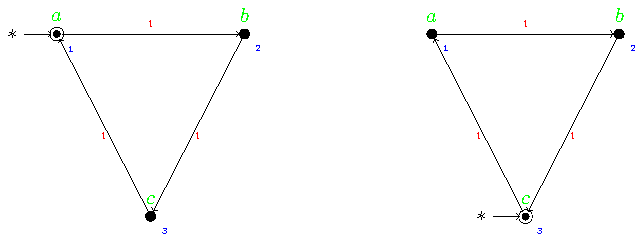
\includegraphics[scale=0.7]{images/counterexample.pdf}
	\caption{Two TGs, $Q$ (left) and $R$ (right), having a different set of traces but the same embedding representation.}\label{fig:counterexample}
\end{figure}
%\begin{example}
%	If we use $\epsilon$ (or $\epsilon^2$) and $\nu$ (or $\nu^2$) for $\phi_{\mathcal{P}}$, we might have a false positive for ``weak equality'' if $Q=(s,s,L,R,w)$ and $R=(s',s',L,R,w)$ are both cycle graphs with $s\neq s'$, $\textit{label}(s)\neq\textit{label}(s')$, $\textit{label}(s)\neq\tau$, and $\textit{label}(s')\neq\tau$. An intuitive example of such situation is presented in Figure \ref{fig:counterexample}: both graphs will have the same frequency for both subtraces and nodes, and therefore have the same  $\epsilon$ and $\nu$ by construction. By having different initial and accepting node with  different labels, we have $\mathcal{W}_0^{\aleph_0}(Q)=\Set{\textup{a(bca)}^n|n\in\mathbb{N}}$ and $\mathcal{W}_0^{\aleph_0}(R)=\Set{\textup{c(abc)}^n|n\in\mathbb{N}}$, thus implying $\mathcal{W}_0^{\aleph_0}(Q)\neq\mathcal{W}_0^{\aleph_0}(R)$ but $k_{\phi_{\mathcal{P}}}(Q,R)=1$ for $t_f=1$.
%\end{example}
%
%
%\begin{lemma}[Weak Equality]
%	Given two TGs $P=(s,t,L,R,w)$ and $P'=(s',t',L',R',w')$ providing the same set of weighted traces, then $k_{\phi_{\mathcal{P}}}(P,P')=ww'$ for $t_f=1$.
%\end{lemma}
%%\begin{proof}
%%	\xout{Given Proposition \ref{lem:rewritinglemma} and the positive definition of $\epsilon$ and $\nu$,  we have that $\norm{\hat{\epsilon}-\hat{\epsilon}'}{2}\to 0$ as well as $\norm{\hat{\nu}-\hat{\nu}'}{2}\to 0$, for which we can immediately close the goal.}
%%\end{proof}
%
%%\xout{As per previous observations, we know that}
%Two TGs should have the maximum dissimilarity when all the non $\tau$-nodes have different labels, thus making it impossible to find an alignment, thus implying that they share an utterly dissimilar set of weighted traces:
%
%\begin{lemma}[Strong Dissimilarity]
%	Given two TGs $P=(s,t,L,R,w)$ and $P'=(s',t',L',R',w')$, $k_{\phi_{\mathcal{P}}}(P,P')=0$ iff. $P$ and $P'$ have a different set of labels with $t_f,w,w'>0$.
%\end{lemma}
%%\begin{proof}
%%	\xout{If we exclude the trivial conditions $t_f=0$, $w=0$ or $w'=0$, the only condition when the kernel returns zero is when  $\Braket{\hat{\epsilon},\hat{\epsilon}'}=0$ and $\Braket{\hat{\nu},\hat{\nu}'}=0$. This implies that, when a component of $\epsilon$ (or $\nu$) is non-zero, the same component of $\epsilon'$ (or $\nu'$) is zero and viceversa. This directly requires that there is a different set of labels associated to the nodes. }
%%\end{proof}
%
%As a corollary of the two lemmas, we have that the proposed embedding performs weakly-ideally as defined in \S\ref{subsec:katk}, as equality condition holds in a relaxed form.
%
%Last, under the assumption that a TG is approximately characterized by $\epsilon$ and $\nu$, we might expect that the TG similarity is characterized by the sum of the distance of both embeddings. Therefore, we show that an increase in both distance embeddings approximately corresponds to a decrease in the kernel output and vice-versa.
%
%\begin{lemma}\label{lem:approxRank}
%	Given two TGs $P=(s,t,L,R,w)$ and $P'=(s',t',L',R',w')$ having respectively the embeddings $(\epsilon,\nu)$ and $(\epsilon',\nu')$, we have that the kernel $k_{\phi_{\mathcal{T}}}$ induces an inverse ranking of $\norm{\hat{\epsilon}-\hat{\epsilon}'}{2}+\norm{\hat{\nu}-\hat{\nu}'}{2}$:
%	$$k_{\phi_{\mathcal{T}}}(P,P')\appropto 2-(\norm{\hat{\epsilon}-\hat{\epsilon}'}{2}+\norm{\hat{\nu}-\hat{\nu}'}{2})$$
%\end{lemma}
%%\begin{proof}
%%	\xout{Let us use $T=t_f^{|R>0|+|R'>0|}$, $\omega=ww'$, $V=\norm{\hat{\nu}-\hat{\nu}'}{2}$, and $E=\norm{\hat{\epsilon}-\hat{\epsilon}'}{2}$ as shorthands. The goal can be rewritten as $k_{\phi_{\mathcal{T}}}(P,P')\appropto 2-(E+V)$. Given that the embeddings $(\epsilon,\nu)$ and $(\epsilon',\nu')$ are normalized kernel function $k_{\phi_{\mathcal{P}}}$ and that they are always positive definite, then we have that $0\leq E +V\leq 2$, so $0\leq 2-(E+V)\leq 2$. Using Proposition \ref{lem:rewritinglemma}, we can write $k_{\phi_{\mathcal{P}}}(P,P')$ as follows:}
%%	$$\Rcancel{\left(1-\frac{E}{2}\right)\omega T+\left(1-\frac{V}{2}\right)T=T\left(\omega+1-\frac{E\omega+V}{2}\right)}$$
%%	\xout{Given that the embeddings $(\epsilon,\nu)$ and $(\epsilon',\nu')$ are normalized in $k$ and that they are always positive definite,  we also have that $0\leq E\omega +V\leq 2$ where $0\leq \omega\leq 1$. We can also write  $0\leq \omega+1-\frac{E\omega+V}{2}\leq \frac{2}{T}$. For $\omega,T=1$, we have that $k_{\phi_{\mathcal{P}}}(P,P')=2-\frac{(E+V)}{2}$. Thus, $0<\omega,T<1$ approximates the expected ranking. }
%%\end{proof}
%
%%\ADD{Such lemma is going to be empirically evaluated in our experiment section.}
